\documentclass[12pt,dvipsnames]{article}

\usepackage{amsmath,amsthm,amssymb,amsbsy}
\usepackage[spanish,es-tabla]{babel}
\decimalpoint
\usepackage{braket}
\usepackage{color}
\usepackage{enumitem}
\usepackage{fancyhdr}
\usepackage{float}
\usepackage[T1]{fontenc}
\usepackage[margin=1.5cm]{geometry} 
\usepackage{graphicx}
\graphicspath{ {images/} }
\usepackage{hyperref}
\usepackage[utf8]{inputenc}
\usepackage{listings}
\usepackage{lmodern}
\usepackage{multicol}
\usepackage{multirow}
\usepackage{pgfplots}
\usepackage{tabularx}
\usepackage{tcolorbox}
\tcbuselibrary{listings,breakable}
\usepackage{tikz}
\usetikzlibrary{babel}
\usepackage{url}
\usepackage{wrapfig}
\usepackage{xcolor}

\setlength{\parindent}{1em}
\setlength{\parskip}{1em}

\definecolor{NARANJA}{rgb}{1,0.467,0}
\definecolor{VERDE}{rgb}{0.31,1,0}
\definecolor{AZUL}{rgb}{0,0.53,1}
\definecolor{ROJO}{rgb}{1,0,0}

\hypersetup{
    colorlinks=true,
    linkcolor=ROJO,
    filecolor=magenta,      
    urlcolor=AZUL,
}
 
\pgfplotsset{compat=1.15}
 
 \renewcommand{\figurename}{Figura}

\renewcommand{\indexname}{Índice}
\renewcommand{\appendixname}{Apéndice}
\renewcommand{\contentsname}{Contenidos}
\renewcommand{\proofname}{Dem.}
\renewcommand{\tablename}{Tabla.}
\renewcommand\qedsymbol{$\blacksquare$}
\newtheorem{teo}{Teorema}[section]
\newtheorem{cor}{Corolario}[section]
\newtheorem{lem}{Lema}[section]
\newtheorem{defi}{Definición}[section]
\newtheorem{obs}{Observación}[section]
\newtheorem{prop}{Propiedades.}[section]
\newtheorem{ejem}{\textbf{\textit{$\circ \ \text{Ejemplo}$}}}[section]
\newtheorem{axi}{Axioma}[section]

\numberwithin{equation}{section}

%%%%%%%%%%%%%%%%%%%%%%%%%%%%%%%%%%%%%%%%%%%%%%%%%%%%%cajas

\newtcolorbox{post}{colback=white,colframe=red!50!black,
	colbacktitle=red!75!black, title= Postulado.}

\newtcolorbox{enu}{colframe=white!85!black, colback=white, leftrule = 10mm, sharp corners, breakable}

\newtcolorbox{solu}{colframe=black, colback=white, leftrule = 1mm, rightrule = -1mm,toprule = -1mm, bottomrule=-1mm, sharp corners, breakable}

\newtcolorbox{corre}{colframe=red, colback=white, leftrule = 1mm, rightrule = -1mm,toprule = -1mm, bottomrule=-1mm, sharp corners, breakable}

\newtcolorbox{enun}{colframe=gray, colback=white!90!black, leftrule = 1mm, rightrule = 1mm, toprule = -1mm, bottomrule=-1mm, sharp corners, breakable}

%%%%%%%%%%%%%%%%%%%%%%%%%%%%%%%%%%%%%%%%%%%%%%%%%%%%%cajas

%%%%%%%%%%%%%%%%%%%%%%%%%%%%%%%%%%%%%%%%%%%%%%%%%%%%%demarcado de soluciones

%New colors defined below
\definecolor{codegreen}{rgb}{0,0.6,0}
\definecolor{codegray}{rgb}{0.5,0.5,0.5}
\definecolor{codepurple}{rgb}{0.58,0,0.82}
\definecolor{backcolour}{rgb}{0.95,0.95,0.92}

%Code listing style named "mystyle"
\lstdefinestyle{mystyle}{
	backgroundcolor=\color{backcolour},   commentstyle=\color{codegreen},
	keywordstyle=\color{magenta},
	numberstyle=\tiny\color{codegray},
	stringstyle=\color{codepurple},
	basicstyle=\ttfamily\footnotesize,
	breakatwhitespace=false,         
	breaklines=true,                 
	captionpos=b,                    
	keepspaces=true,                 
	numbers=left,                    
	numbersep=5pt,                  
	showspaces=false,                
	showstringspaces=false,
	showtabs=false,                  
	tabsize=2
}

%"mystyle" code listing set
\lstset{style=mystyle}

\newenvironment{sol}{\begin{figure}[H]
		\begin{tikzpicture}
		\filldraw[black] (0,0) circle (3pt);
		\draw[line width = 0.5pt] (0,0) -- (4,0) node[above right]{\textbf{Solución:}};
		\end{tikzpicture}
\end{figure}}{\begin{figure}[H]
		\begin{flushright}
			\begin{tikzpicture}
			\draw[line width = 0.5pt] (0,0)-- (4,0);
			\filldraw (4,0) circle (3pt);
			\end{tikzpicture}
\end{flushright}\end{figure}}

%%%%%%%%%%%%%%%%%%%%%%%%%%%%%%%%%%%%%%%%%%%%%%%%%%%%%demarcado de soluciones
 
\begin{document}

\title{Ortogonalización y ortonormalización \\ (Teorema de Gram-Schmidt)}
\date{}
\maketitle
%\tableofcontents

\begin{obs}\label{obs:1}
    Hemos visto ya la utilidad de las bases ortogonales y ortonormales \textemdash y, a través de ellas, la interpretación del producto escalar y la norma inducida\textemdash \ sin, hasta el momento, haber justificado su existencia. En este video, mostraremos cómo a partir de un conjunto linealmente dependiente finito se puede producir un conjunto ortogonal linealmente independiente u ortonormal que genere el mismo subespacio vectorial. Este resultado se conoce como el Teorema de Gram-Schmidt, y un corolario de este teorema es que las bases ortogonales y ortonormales siempre existen en espacios vectoriales con producto escalar de dimensión finita.
\end{obs}

\begin{obs}
Siguiendo de la observación \ref{obs:1}, las ideas principales a presentar en este video son:

\begin{enumerate}[label=(\roman*)]
    \item En un espacio vectorial real, a partir de cualquier conjunto linealmente independiente de dos vectores se puede obtener \textemdash mediante la modificación de uno de ellos con las operaciones de suma vectorial, producto de un vector por un escalar, y producto escalar\textemdash \ un conjunto ortogonal linealmente independiente que genere el mismo subespacio vectorial que el conjunto original (de hecho, se pueden obtener dos, dependiendo de cuál de los vectores modificamos), y lo mismo para conjuntos ortonormales.
    
    \item En un espacio vectorial real, a partir de cualquier conjunto linealmente independiente de tres vectores se puede obtener un conjunto ortogonal linealmente independiente que genere el mismo subespacio vectorial que el conjunto original (de hecho, se pueden obtener seis, dependiendo de cuál de ellos no modificamos), y lo mismo para conjuntos ortonormales.

    \item En un espacio vectorial arbitrario, a partir de cualquier conjunto linealmente independiente finito se pueden obtener conjuntos ortogonales linealmente independientes que generen el mismo subespacio que el conjunto original \textemdash y lo mismo para conjuntos ortonormales \textemdash \ mediante procesos algorítmicos finitos. Como consecuencia, todos los espacios vectoriales con producto escalar de dimensión finita tienen bases ortogonales y ortonormales.
\end{enumerate}
\end{obs}

%%%%%%%%%%%%%%%%%%%%%%%%%%%%%% PRIMERA ESCENA %%%%%%%%%%%%%%%%%%%%%%%%%%%%%

\newpage
\section{Primera escena}

Supongamos que, en un espacio vectorial real con producto escalar, tenemos un conjunto de dos vectores linealmente independientes\footnote{Mostramos brevemente que están en ejes distintos.}, pero no ortogonales entre sí, y que queremos modificar a alguno de ellos, utilizando las operaciones disponibles\footnote{Mostramos brevemente algo como $\vec{u}+\vec{v}, a\vec{u}, \langle\vec{u},\vec{v}\rangle$ en pantalla, para que se entienda que nos referimos a las operaciones de suma vectorial, producto de un vector por un escalar y producto escalar.}, de tal forma que obtengamos un conjunto de dos vectores linealmente independientes y \emph{ortogonales} que genere el mismo subespacio vectorial que el conjunto original\footnote{Mostramos que $\langle I\rangle$ es todo el plano.}, el cual mostraremos a continuación.

Por definición, el hecho de que nuestros vectores $\vec{a}$ y $\vec{b}$ no sean ortogonales significa que su producto escalar es distinto de cero\footnote{Mostramos $\langle \vec{a},\vec{b}\rangle\neq0$ en pantalla.}, por lo que la proyección vectorial\footnote{Hacemos dos proyecciones vectoriales rápidas para mostrar que, en efecto, son no nulas.} de $\vec{a}$ sobre $\vec{b}$ es distinta del vector nulo. Observemos que, debido a la propiedad\footnote{Debajo de $\langle\vec{a},\vec{b}\rangle\neq0$, mostramos brevemente $\langle \vec{b},\vec{a}\rangle = \overline{\langle \vec{a},\vec{b}\rangle}$ y, abajo, $\implies \langle\vec{b},\vec{a}\rangle\neq0$ (quedaría como un silogismo); luego, desaparecemos los tres renglones, junto con la proyección vectorial de $\vec{a}$ sobre $\vec{b}$.} de simetría conjugada del producto escalar, se sigue que la proyección vectorial de $\vec{b}$ sobre $\vec{a}$ también es no nula y, por ende, que cada uno de los vectores debe tener una componente no nula en el subespacio generado por el otro vector.

¿Qué pasa si le removemos\footnote{Usamos la proyección vectorial de $\vec{b}$ sobre $\vec{a}$ para ortogonalizar a $\vec{b}$, obteniendo así a $\vec{b}'$, y escribimos $\Gamma_1=\{\vec{a},\vec{b}'\}$.} esta componente a uno de los vectores? Obtenemos un conjunto ortogonal, ¡como queríamos! Veamos que este conjunto ortogonal efectivamente \emph{genera el mismo subespacio vectorial que el conjunto linealmente independiente con el que empezamos}\footnote{Mostramos al generado de $\Gamma_1$ (que es todo el plano) y escribimos $\langle \Gamma_1 \rangle = \langle I \rangle$ en pantalla.}; esto se debe a que obtuvimos al vector $\vec{b}'$ como combinación lineal de los vectores de $I$ y, además, a que los vectores claramente no perdieron su independencia lineal\footnote{Trazamos líneas punteadas para mostrar que los vectores ortogonalizados están ejes distintos.} cuando los ortogonalizamos de esta forma.

Observemos que\footnote{Regresamos al conjunto $I$ original con las dos proyecciones vectoriales, desaparecemos ahora a la proyección vectorial de $\vec{b}$ sobre $\vec{a}$ y usamos la de $\vec{a}$ sobre $\vec{b}$ para ortogonalizar a $\vec{a}$ y obtener así a $\vec{a}'$.}, si partiendo de nuestro conjunto original hubiéramos decidido modificar al \emph{otro} vector de manera análoga, entonces hubiéramos obtenido un conjunto ortogonal \emph{distinto}\footnote{Escribimos $\Gamma_2=\{\vec{a}',\vec{b}\}$ en pantalla.} al anterior pero que, nuevamente, genera el \emph{mismo} subespacio\footnote{Mostramos al generado de $\Gamma_2$ (nuevamente, todo el plano) y escribimos $\langle \Gamma_1 \rangle = \langle I \rangle=\langle \Gamma_2 \rangle$ en pantalla.} que el conjunto original. Si quisiéramos hacer que este conjunto fuese ortonormal, podríamos simplemente normalizar a cada uno de los vectores\footnote{Tomamos el conjunto ortogonal que ya tenemos y normalizamos a cada uno de los vectores; luego, hacemos \emph{fade out}.}. Sin embargo, si nuestro objetivo hubiera sido obtener un conjunto ortonormal desde el principio\footnote{Borramos todo y dejamos sólamente al conjunto l.i. original y el texto $I=\{\vec{a},\vec{b}\}$.}, entonces, recordando que es más sencillo calcular proyecciones vectoriales sobre vectores unitarios, pudimos haber empezado\footnote{Esta vez, empezamos normalizando a $\vec{b}$ para definir a $\hat{b}$, luego ortogonalizamos a $\vec{a}$ proyectándolo sobre $\hat{b}$, obteniendo así a $\vec{a}'$, y lo normalizamos para definir a $\hat{a}'$; finalmente, escribimos $N=\{\hat{a}',\hat{b}\}$.} el proceso normalizando a uno de los vectores y, luego, removiéndole al \emph{otro} vector su componente a lo largo del eje del vector normalizado, y normalizándolo también. Una vez más, observemos que el subespacio generado\footnote{Mostramos al generado de $N$ y escribimos $\langle I\rangle=\langle N\rangle$.} por este conjunto \emph{ortonormal} es igual al generado por el conjunto linealmente independiente original.

%%%%%%%%%%%%%%%%%%%%%%%%%%%%%% SEGUNDA ESCENA %%%%%%%%%%%%%%%%%%%%%%%%%%%%%

\newpage
\section{Segunda escena}

Consideremos ahora a un espacio vectorial real con producto escalar con un conjunto de tres vectores linealmente independientes pero no ortogonales entre sí. Veamos el subespacio generado por este conjunto. ¿Cómo podríamos obtener un conjunto linealmente independiente y ortogonal de tres vectores a partir del conjunto que tenemos, de tal forma que el subespacio generado no cambie?\footnote{Tal vez poner un ¿? grande y divertido en pantalla jiji} Sugerimos pausar el video\footnote{Dejamos el espacio rotando unos segundos de tal forma que, cuando empiece el siguiente párrafo, ya se encuentre en una posición conveniente para empezar a hacer las proyecciones/modificaciones.} para pensar cómo modificarías a estos tres vectores para cumplir nuestro objetivo, y continuar la reproducción hasta que tengas una idea clara \textemdash y, de preferencia, escrita\textemdash \ de cómo hacerlo.

Iniciamos de la misma manera: escogemos a un vector de referencia, por ejemplo, el vector $\vec{a}$; proyectamos a otro vector \textemdash digamos, a $\vec{b}$\textemdash \ sobre $\vec{a}$ y restamos esa componente a $\vec{b}$, obteniendo así un conjunto linealmente independiente y ortogonal de dos vectores\[
\{\vec{a},\vec{b}'\}.
\] De la misma manera, tomamos al vector restante $\vec{c}$ y le removemos su componente a lo largo del eje del vector $\vec{a}$; de esta forma, aseguramos que este nuevo vector sea ortogonal al vector $\vec{a}$; sin embargo, esto no necesariamente implica que también sea ortogonal a $\vec{b}'$. Por ende, además de removerle a $\vec{c}$ su componente a lo largo del eje de $\vec{a}$, debemos removerle su componente a lo largo del eje de $\vec{b}'$. De esta forma, aseguraremos que el conjunto compuesto por $\vec{a}$, $\vec{b}'$ y $\vec{c}'$ sea ortogonal y linealmente independiente\footnote{Escribimos ``*Ver el Ejercicio 3.1 al final del video.''.}. Observemos que este nuevo conjunto genera el mismo subespacio vectorial que el conjunto original.
\[
\Gamma_1 = \{\vec{a},\vec{b}',\vec{c}'\}.
\]

Hacemos énfasis en que, habiendo elegido un vector de referencia \textemdash como el vector $\vec{a}$\footnote{Mostramos dos copias del mismo conjunto $l.i.$ arriba y abajo (sin nombres), resaltamos al mismo vector (de referencia), ortogonalizamos en diferente orden y escribimos $\Gamma_1$ y $\Gamma_2$.}, en el ejemplo anterior\textemdash, si cambiamos el orden en el que modificamos a los demás vectores, obtendremos también un conjunto ortogonal y linealmente independiente, aunque puede ser distinto al que obtuvimos anteriormente. Lo mismo ocurre si elegimos a cualquier otro vector como vector de referencia\footnote{Hacemos algo análogo para $\Gamma_3$ y $\Gamma_4$ y, luego, para $\Gamma_5$ y $\Gamma_6$.}. No es difícil ver que cualquiera de estos conjuntos ortogonales generará el mismo subespacio vectorial que el conjunto original.

Nuevamente, si desde el principio nuestro objetivo hubiera sido obtener un conjunto \emph{ortonormal} de tres vectores, pudimos haber empezado por normalizar a uno de los vectores, después, proyectar a alguno de los otros vectores sobre el vector normalizado, remover esa componente y normalizar al vector resultante y, finalmente, proyectar al último vector sobre los dos vectores normales que tenemos, removiendo dichas componentes y normalizando al vector resultante\footnote{En este párrafo ya no se hacen referencias a vectores con un nombre específico, pues en el párrafo pasado ya se estableció que tanto el punto como de partida como el orden es arbitrario; la animación debería reforzar este hecho quitándole los nombres a los vectores. Conceptualmente, esto facilita la transición a la escena tres.}.

%%%%%%%%%%%%%%%%%%%%%%%%%%%%%% TERCERA ESCENA %%%%%%%%%%%%%%%%%%%%%%%%%%%%%

\newpage
\section{Tercera escena}

Este procedimiento para, a partir de un conjunto linealmente independiente de dos o tres vectores, obtener conjuntos linealmente independientes y \emph{ortogonales} que generen el mismo subespacio que el conjunto original puede ser generalizado para conjuntos finitos de cualquier cardinalidad, y se conoce como el proceso de Gram-Schmidt. Lo mismo ocurre con el procedimiento que nos permite obtener conjuntos \emph{ortonormales} sin cambiar el subespacio generado. Éste es conocido como el proceso de Gram-Schmidt \emph{modificado}\footnote{En esta imagen faltó agregar $<\Gamma>=<I>=<N>$ centrado debajo de donde dice 5 (aparecería hasta el final).}. A continuación, enunciaremos ambos procesos de forma matemática. Sugerimos comparar esto con la versión escrita vista anteriormente. 

\begin{figure}[h!]
    \centering
    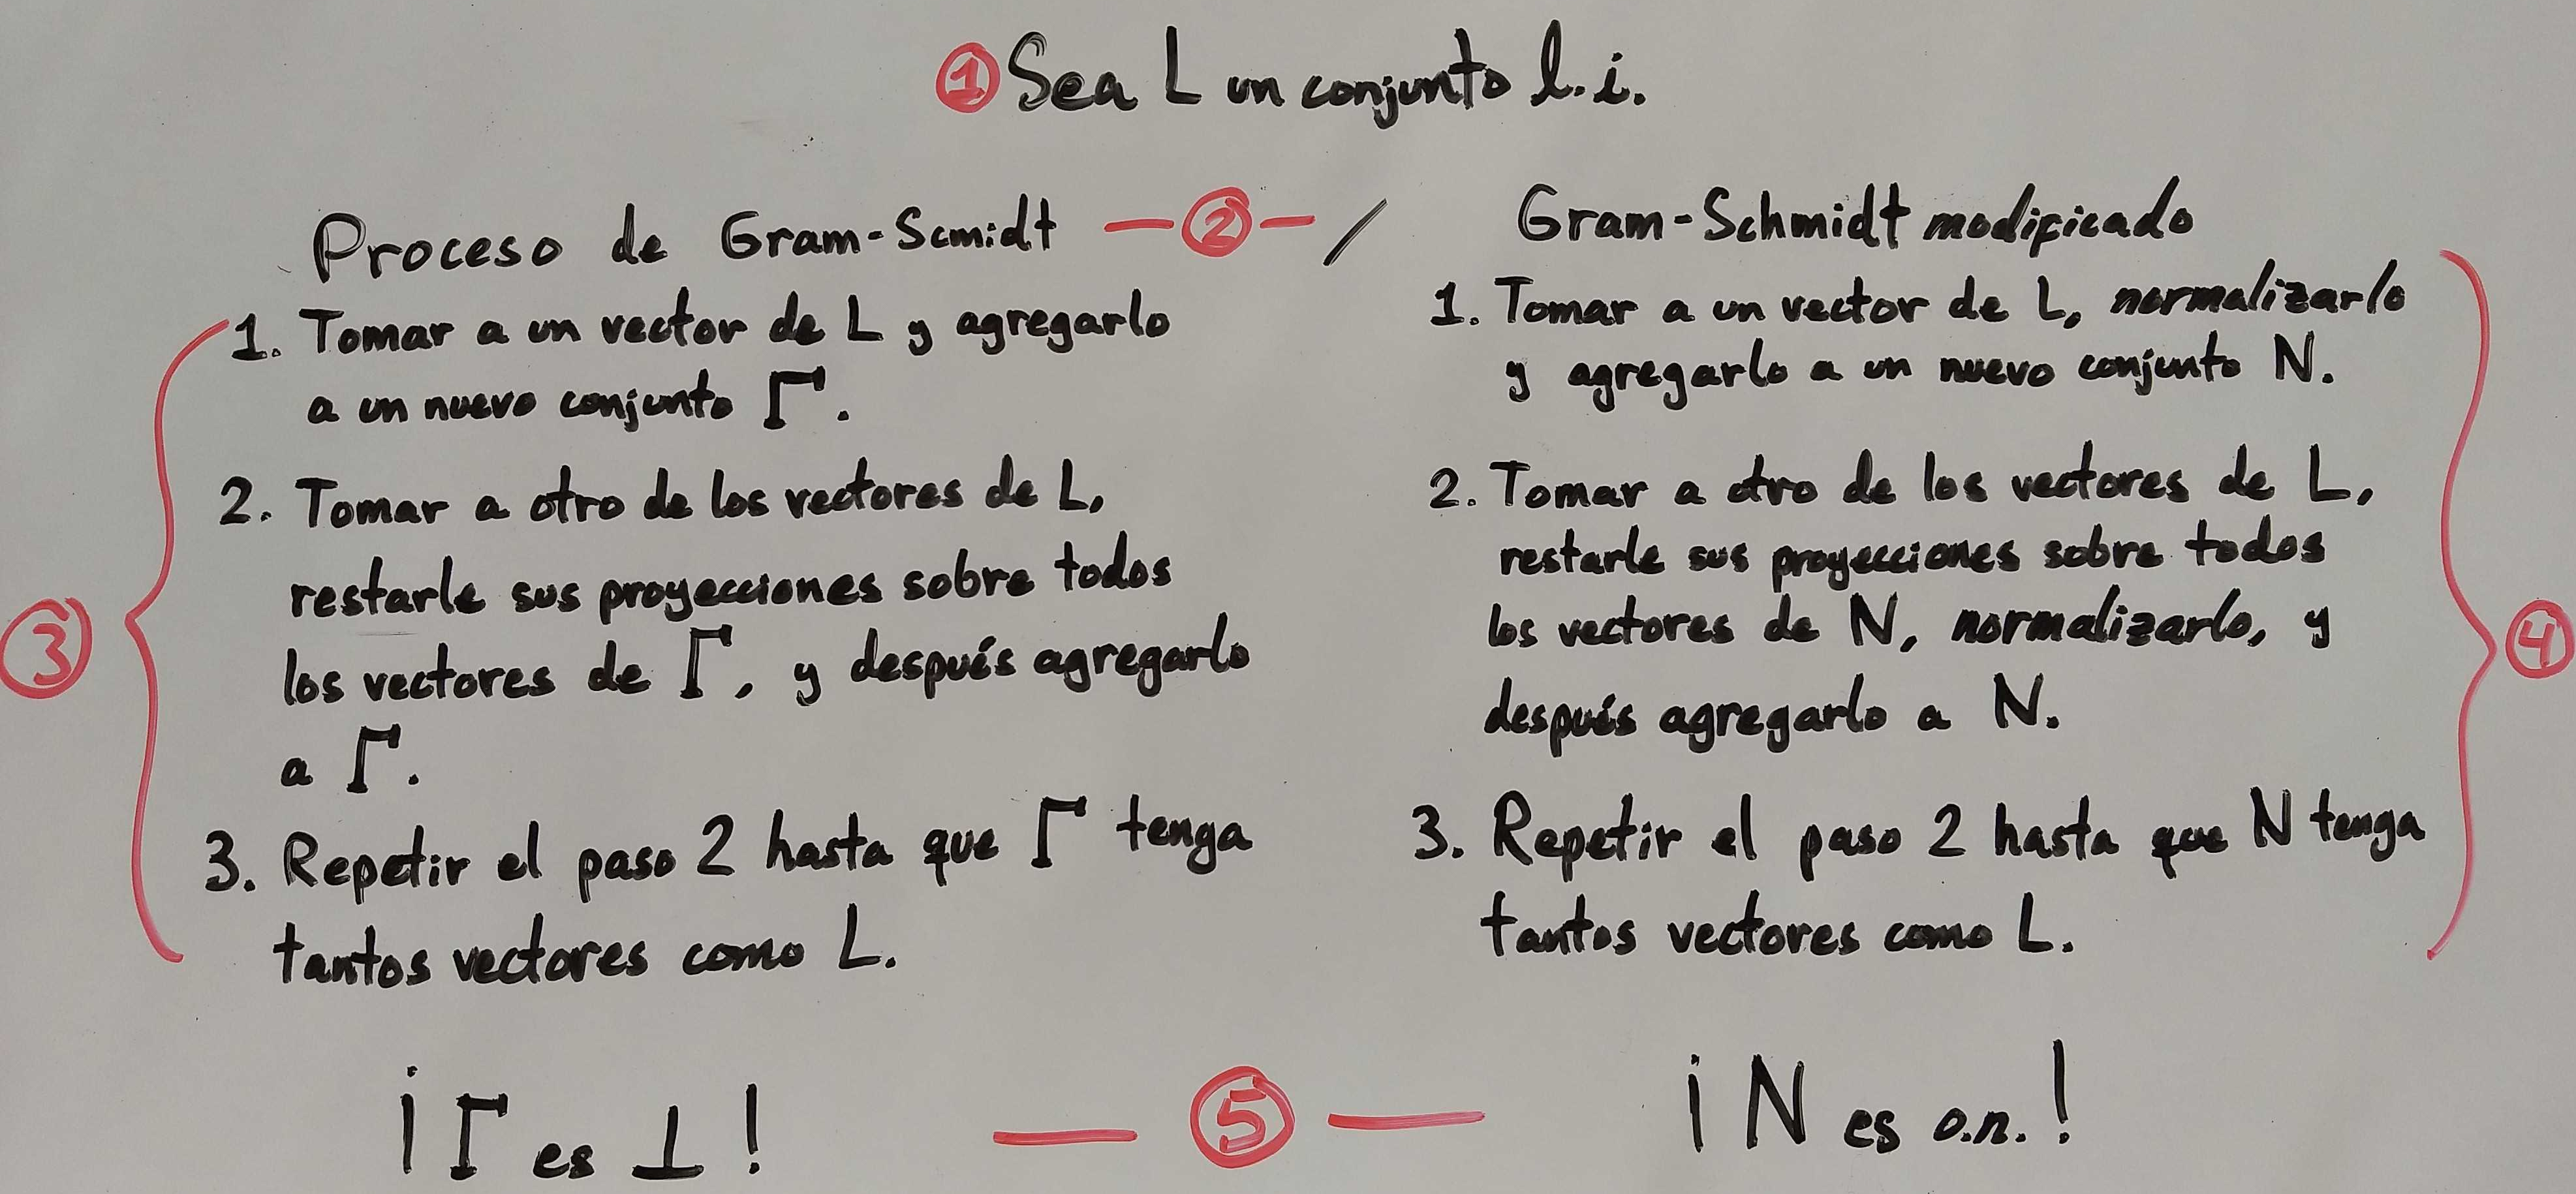
\includegraphics[width=16cm]{1.png}
\end{figure}

En conjunto, este resultado se conoce como el Teorema de Gram-Schmidt. Observemos que, como consecuencia de este teorema, se sigue que la existencia de bases ortogonales y ortonormales siempre está asegurada en los espacios vectoriales con producto escalar de dimensión finita\footnote{Mejor porner los vectores ``n''s con gorritos ya que, por la forma en que los estamos definiendo, son unitarios, y el objetivo es que la base $N$ sea ortonormal.}.

\begin{figure}[h!]
    \centering
    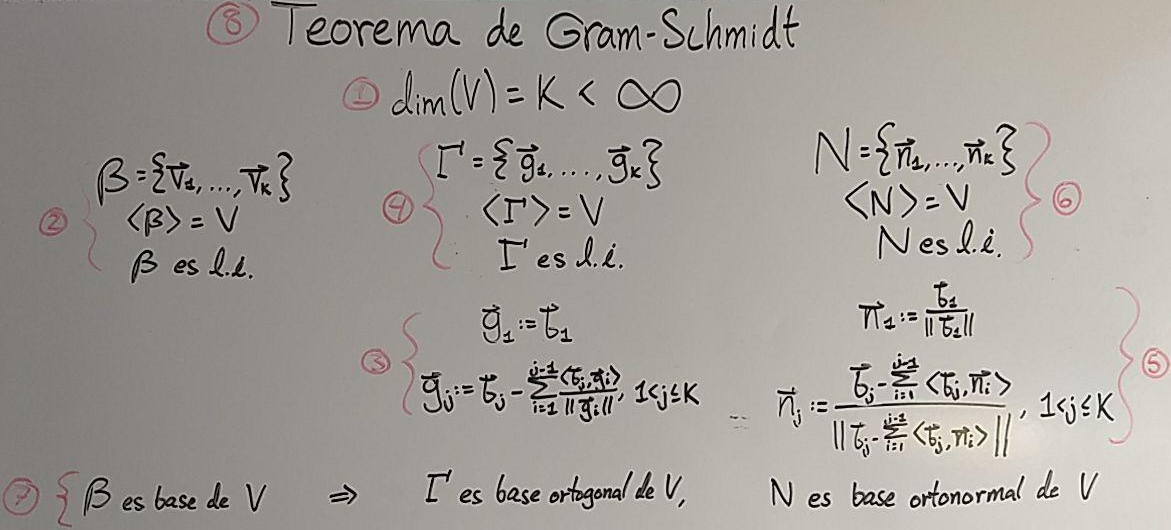
\includegraphics[width=16cm]{2.png}
\end{figure}


%%%%%%%%%%%%%%%%%%%%%%%%%%%%%% ÚLTIMA ESCENA %%%%%%%%%%%%%%%%%%%%%%%%%%%%%

\newpage
\section{Escena final}

Ejercicio 3.1 Sea $V$ un espacio vectorial con producto escalar. Demuestra que
\begin{align*}
    \bigg\langle \vec{u}, \vec{v} - \frac{\langle \vec{v}, \vec{u}\rangle}{\langle \vec{u} , \vec{u} \rangle}\vec{u} \bigg\rangle = 0 \quad \text{y} \quad \bigg\langle \bigg\{\vec{u}, \vec{v} - \frac{\langle \vec{v}, \vec{u}\rangle}{\langle \vec{u} , \vec{u} \rangle}\vec{u} \bigg\} \bigg\rangle = \langle \{\vec{u}, \vec{v}\} \rangle
\end{align*} para $\vec{u},\vec{v}\in V$ con $\vec{u},\vec{v}\neq\vec{0}$, y dibuja un ejemplo en $\mathbb{R}^2$.\footnote{En la descripción del video o en los comentarios podemos poner la siguiente ``Pista: Para la primera parte, utiliza el Ejercicio 1.1.''.}\\

Ejercicio 3.2 Usa la intuición geométrica generada por este video para demostrar el Teorema de Gram-Schmidt.\\

Pregunta 3.3 ¿Qué sucedería si aplicáramos el proceso de Gram-Schmidt a un conjunto de vectores linealmente \emph{dependiente}?\footnote{Respuesta: obtendríamos un conjunto ortogonal linealmente independiente con tantos vectores como vectores linealmente independientes haya tenido el conjunto original.} \\

Pregunta 3.4 ¿Qué sucedería si, en el proceso de Gram-Schmidt modificado, normalizáramos a alguno de los vectores \emph{antes} de ortogonalizarlo, y no \emph{después}?\footnote{Respuesta: los vectores obtenidos no serían unitarios, por lo que el conjunto resultante no sería ortonormal.} \\

Pregunta 3.5 El Teorema de Gram-Schmidt \textbf{no} asegura la existencia de bases ortogonales y ortonormales en espacios vectoriales con producto escalar de dimensión \textbf{infinita}, ¿por qué?\footnote{Respuesta: porque las combinaciones lineales infinitas, en general, no están bien definidas.} (Sugerencia: piensa en la Pregunta 1.2.)

\end{document}
